\footnotesize
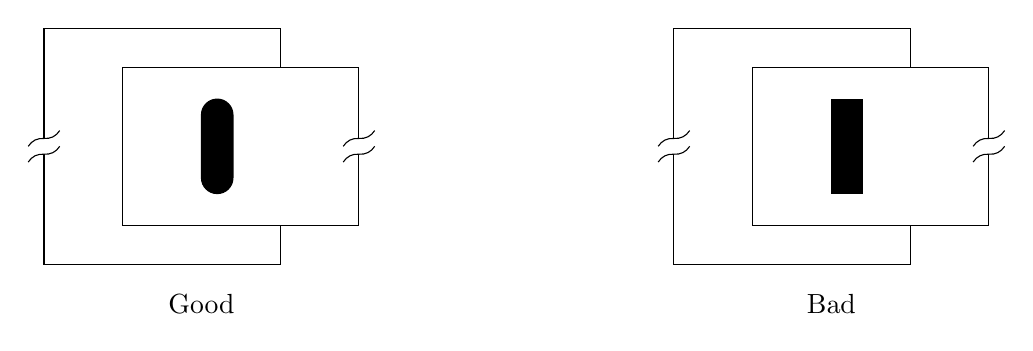
\begin{tikzpicture}[scale=1,ext/.pic={
\path[fill=white](-0.2,0)to[bend left](0,0.1)to[bend right](0.2,0.2)to(0.2,0)to[bend left](0,-0.1)to[bend right](-0.2,-0.2)--cycle;
\draw(-0.2,0)to[bend left](0,0.1)to[bend right](0.2,0.2) (0.2,0)to[bend left](0,-0.1)to[bend right](-0.2,-0.2);
}]
\draw(2,-1.5)rectangle(-1,1.5);
\draw[fill=white](0,-1)rectangle(3,1);
\draw(3,0)pic{ext};
\draw(-1,0)pic{ext};
\draw[rounded corners=2mm,fill=black](1,-.6)rectangle++(.4,1.2);
\node at(1,-2){Good};
\begin{scope}[xshift=8cm]
\draw(2,-1.5)rectangle(-1,1.5);
\draw[fill=white](0,-1)rectangle(3,1);
\draw(3,0)pic{ext};
\draw(-1,0)pic{ext};
\draw[fill=black](1,-.6)rectangle++(.4,1.2);
\node at(1,-2){Bad};
\end{scope}
\end{tikzpicture}